\documentclass[12pt,notitlepage]{article}
\usepackage[utf8]{inputenc}
\usepackage[english]{babel}
% \usepackage[margin=1.0in]{geometry}
\usepackage{graphicx}
% \usepackage[pdftex]{hyperref}
% \usepackage{csquotes}
% \usepackage{titling}
% \usepackage{titlesec}
% \usepackage{xspace}
% \usepackage{tabularx}
\usepackage{float}
% \usepackage{parskip}

\usepackage[backend=bibtex,style=numeric]{biblatex}
\bibliography{references}

% Title Page
\title{Height Field Water Simulation}
\author{Joseph Wilson, Arnaud Filliat, and Jacob Davis}
\date{\today}

\begin{document}

\maketitle

\section{Abstract}

We investigated many ways of simulating water including wave particle systems, 
procedural fluids, and various height fields. Of all the available methods, we 
chose to implement a height field water simulation for two fundamental reasons, 
the ability to run it in real time and the ability to implement realistic 
object interactions. A height field is comprised of a two dimensional array of 
columns that is particularly tailored for simulating fluid wave propagation. 
Our implementation works well for modeling the surface movement of water 
including ripples reflecting off of the boundaries of the height field. It also 
works well for simulating object interactions that affect and are effected by 
the height field. We faced challenges in creating realistic reflection off of 
the boundaries and realistic interactions with a solid object that can both 
affect and respond to the height field through basic kinematics.

\section{Introduction}

Many applications of computer graphics involve fluid simulations of some sort.  The most realistic simulations involve massive particle systems and take large amounts of time to run offline.  For applications that are interactive, this is unreasonable and other solutions must be explored.  Procedural fluids are acceptable for background situations where the user does not actually interact with it but it’s illusion of realism is rapidly destroyed when any object comes in contact with it.  As such it is important to find a solution that allows interaction in real-time with fluids, primarily water.

While many solutions exist most all rely on reducing the complexity of the 
simulation.  Wave particles reduce from a particle for each molecule of water 
to a particle for a wave that deforms the water surface as it passes.  We chose 
to focus on height fields which reduce a 3-dimensional particle system to a 2 
dimensional system of columns.  This provides a massive reduction in 
computational intensity while maintaining an acceptable level of realism in 
most simulations.

\begin{figure}[H]
    \caption{Height Field}
    \label{fig:field}
    \centering
    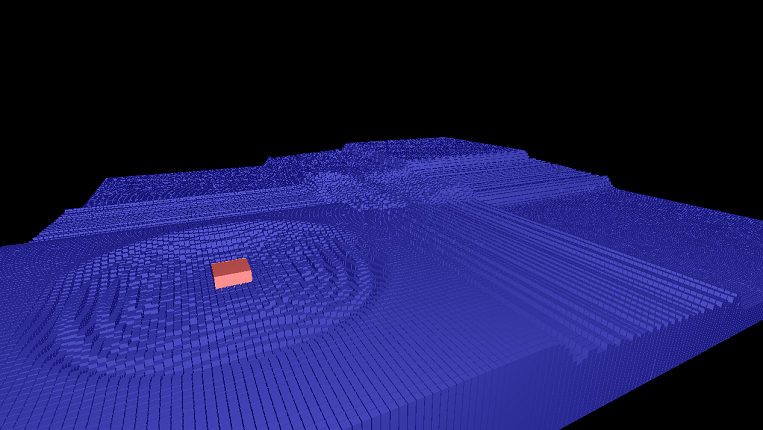
\includegraphics[width=0.5\textwidth]{../www/images/field}
\end{figure}

In this project we implement a height field simulation and give the user the 
ability to drop a cube into the fluid in real-time as show in \ref{fig:field}.  
In this paper we will detail the internals of this implementation and problems 
we encountered.  We will begin, however, by discussing the advantages and 
disadvantages of various types of fluid simulations.

\section{Related Work}

Computational fluid dynamics has a long history. The first development was in 
the 1800s when George Stokes formulated the Navier-Stokes equation which 
describes the dynamics of fluids. Using this equation which describes the 
conservation of momentum and a mass conservation equation and state equation it 
becomes possible to simulate fluids. \cite{particle}
Numerous approaches have been used to describe fluid dynamics on computers. 
Particle-based approaches have been used to animate surfaces, lava flows, and 
animate fluid motion. \cite{smooth}\cite{dynamic}\cite{implicit} Using 
particles can simplify the conservation of mass equation and Navier-Stokes 
equation because the number of particles is constant and each particle has a 
constant mass thus conservation is guaranteed.
Particle systems have been used for things other than fluid simulations too and 
are greatly applicable. A good example is for object modeling. \cite{oriented} 
For fluids 
particle systems can realistically animate fluids and how they interact with 
various objects, yet fall short with larger bodies. \cite{particle}

Another use for particle system is a wave particle method. Wave particle have 
position and mass like all other particles but also store the propagation 
angle, dispersion angle, origin, and amplitude. Using all of these the wave 
particle can give the direction of the wave, the energy of the wave and the 
spatial range in which the particles appear. In this particle system wave 
boundaries are required for reflecting the wave fronts. \cite{realtime} Wave 
particles are similar to how height fields and our system will work yet our 
system should be able to be expanded to a bigger field without loss of 
real-time display due to the low computational overhead.

Another technique used in the past involves shallow water equations. These 
equations also uses the Navier-Stokes equation and are derived by depth 
integrating it. This creates a set of partial differential equations that 
describe the flow below a pressure surface in a fluid.  An interesting point 
about shallow water equations is that the vertical velocity term is not present 
in them yet this does not mean the vertical velocity is zero as otherwise there 
would be no movement in the wave surface. Shallow water equations have been 
used in the past to model Coriolis forces in atmosphere and oceanic models. 
\cite{shalloweq}


\section{Problem Statement}

Simulating water in real-time is very difficult as water is a large particle system where each particle interacts with its neighbors via a complex set of equations.  Very realistic water simulations can be created with particle systems, however, it is not generally reasonable to expect them to run in real-time.  This is due to the large amount of computational power required to update a complex 3-dimensional particle system.  One solution to the problem is wave particles.  Wave particles have a relatively low computational cost as the particles do not have to interact with each other and only have to apply a simple deformation to a plain.  The problem with wave particles is that it is difficult to model many different types of object.  The technique requires a separate set of information for each object resulting in large memory costs with many objects.  Height fields were the solution we chose as they reduced the computational complexity of particle systems to two dimensions while still providing a great deal of realism and the ability to interact with objects relatively easily with minimal comparative computational costs.  Shallow water equations provide a much more realistic simulation than height fields while requiring a minimal amount of extra memory but we were unable to reach a stage where we could implement them.
 
\section{Problem Solution}

Any water simulation has two primary parts, the water movement and the water 
lighting.  Our implementation focuses on water movement.  The height field 
information is stored in two, two dimensional arrays.  One for column height 
and one for column velocity.  These columns are updated each frame.  Each 
column calculates the force on it due to the four surrounding columns with this 
equation. \[ f = c^2 ( u[i+1,j] + u[i-1,j] + u[i,j+1] + u[i,j-1] – 4 u[i,j] 
)/h^2 \]  C 
represents the speed of a wave and h represents the width of a column.  This 
equation is derived from a reduction of realistic wave equations to two 
dimensions.  Our simulation takes place on a large scale with each column 
representing a 1 meter by 1 meter column of water.  After the force is 
calculated, it is applied to the velocity of each column.  The force is 
multiplied by the amount of time that has passed since the last update, 1/60th 
of a second in our case.  This ensures that steps remain constant even if 
framerate is changed.  After all velocities have been updated the height of 
each column is modified by adding velocity multiplied by the time step.  This 
process of forward Euler integration can lead to feedback loops if not 
controlled so we implement damping and clamping.  Velocity is damped by a 
factor of 0.99 each step and column height is bounded between -100 and 100 
although with the damping factor these extremes are rarely reached.

\begin{figure}[H]
    \caption{Reflecting Waves}
    \label{fig:reflection}
    \centering
    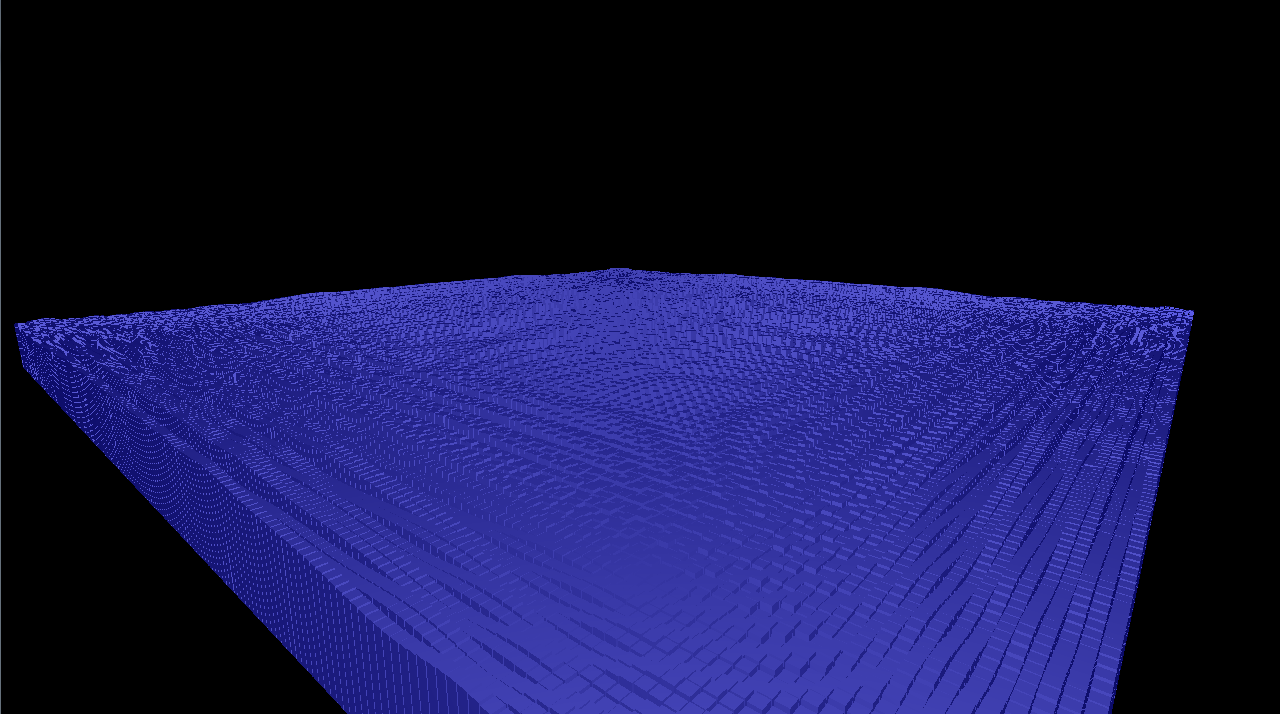
\includegraphics[width=0.5\textwidth]{../www/images/bouncingWaves}
\end{figure}
	
An important part of the simulation is using various boundary conditions to 
mimic realistic wave reflection off of rigid surfaces, as seen in figure 
\ref{fig:reflection}, or mimic large bodies of 
water. Our implementation has the option to perform four different boundary 
conditions using a variety of techniques. The first technique to be implemented 
is called boundary clamping. When using clamping, the columns on the edges of 
the height field use themselves in place of any missing columns. This creates 
an effect similar to water reflecting off of a rigid vertical surface with a 
minimal velocity on columns around the edges of the height field. The next 
technique is called wrapping boundaries. Boundaries that wrap use the columns 
on the opposite side of the height field to calculate their velocities. This is 
useful for creating an effect similar to how water reacts in a large body by 
copying one height field in a checkerboard pattern to easily create a large 
body without having to process an excess of columns which could effect 
framerate. Finally, the last two techniques use a ghost boundary for 
reflecting. These techniques are similar to clamping and perform similarly, but 
instead of a column using itself as a reference when there is no column on one 
or more sides of it, a ghost column is used. In one implementation, the average 
height of the columns in the height field is used creating an extremely rigid 
outer wall of columns around the height field. The other implementation uses 
the slope between the outermost and second most outer columns to determine the 
height of the ghost. This method can be very realistic, but it has one inherent 
flaw. If the heights of the corners of the height field are not equal to the 
average height of all the columns, there will be a slant leading to the corners 
in question. This is because the heights of the corners never changes in this 
implementation due to how they are calculated. There are some simple hacks to 
avoid this such as setting the corners to be equal to the average at the start 
or using clamping only for the corners, but we left this flaw in our program to 
display it.

\begin{figure}[H]
    \caption{Object Creating Ripples}
    \label{fig:ripples}
    \centering
    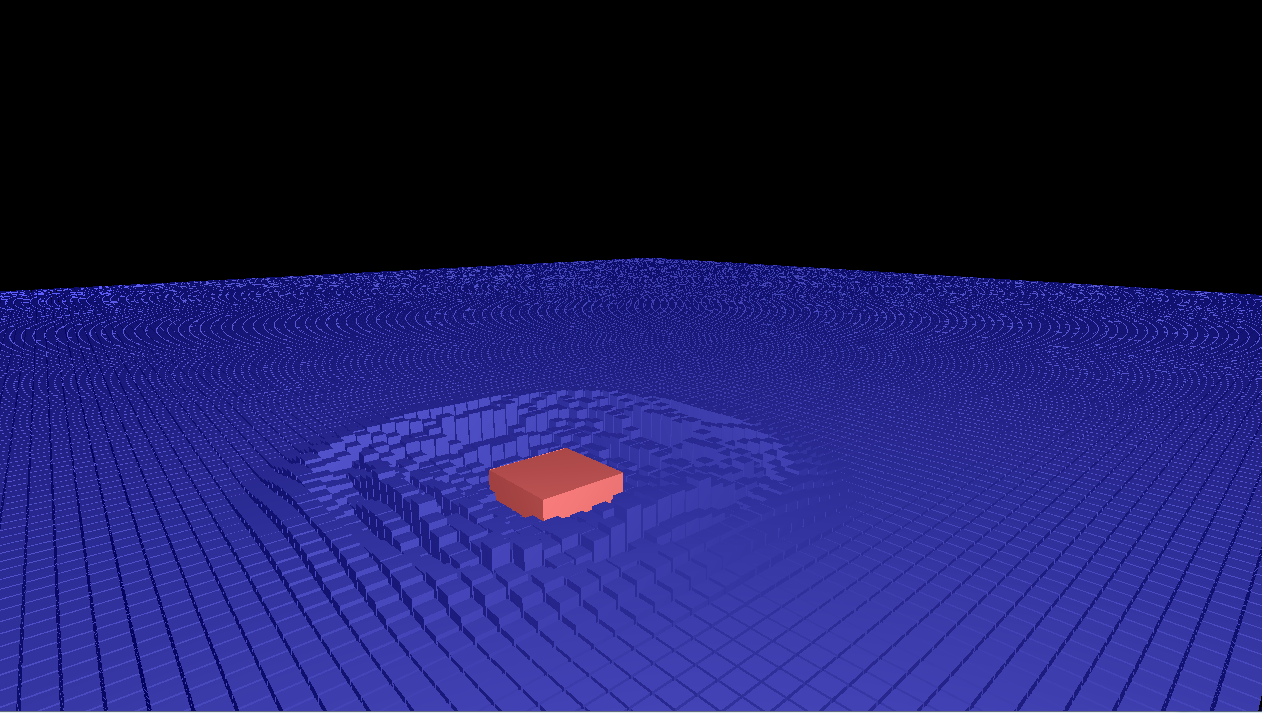
\includegraphics[width=0.5\textwidth]{../www/images/objectRipples}
\end{figure}

Object interaction is implemented with a cube and our cube is drawn with edges 
parallel to the edges of our columns the cube being dropped into the water 
creating ripples can be seen in figure \ref{fig:ripples}.  To create these 
ripples, during each step of 
the simulation we 
find the location of the corners of the cube with respect to the indices of our 
columns.  This allows us to compare the cubes height with that of the water.  
By subtracting the height of the base of the cube from the height of the water 
and clamping between 0 and cube width we calculate the amount of water 
displaced by the cube.  The displacement of each column is stored in another 
2-dimensional array and by comparing the new displacement with the old we are 
able to calculate the change in displacement of water by the cube.  Once the 
total displacement and the change in displacement are known these values are 
used to calculate the force on the cube and the change in water level around 
the cube respectively.  Any change in displaced water is added or subtracted 
directly to the columns surrounding the cube.  Our height field inside the cube 
is not modified allowing water to cover the cube should it fall below the water 
level.  Because the height field is not modified on the inside of the cube a 
feedback loop can occur.  The displaced water is added to the surrounding 
columns which flow inward increasing the amount of displaced water by the cube, 
adding more water to the surrounding columns.  This was solved in two ways.  
The first option sets the height of each internal column to halfway up the 
cube.  This allows the following update due to column velocity to pull a column 
above the cube and prevents the feedback loop but gives the water a much more 
viscous appearance with it clinging to the cube, creating depressions and 
mounds in the surface when the cube is dropped and raised respectively.  The 
second option is to use the average water level instead of the local column 
height.  This leads to realistic simulations when the water is relatively flat 
but leads to disconnected water ripples and cube movement if the surface is far 
above or below average at that location.  Once the water is updated the cube is 
moved using Forward Euler integration and standard physics equations.  Force 
due to water is calculated with density*gravity*displacement and both it and 
gravity are applied to velocity and then velocity to cube location.

It is also important to ensure water is not added or removed from the simulation.  To do this we initially calculate an average volume for a column.  Upon each step we recalculate this average and add or subtract the difference from every column.  This prevents small errors in calculation from drastically altering the volume of our fluid over time.

The final step is drawing the height field.  To do this we created an additional array that contains a point representing the top left corner of each column.  The x and z components were the indices of a location and the y the height.  This array was transferred to the GPU via and VBO and VAO to as points.  A geometry shader then took each point and expanded it into a column, adding sides with specified widths and a height determined by the height of each point.  The columns were then shaded with Blinn-Phong shading.  A simple set of Blinn-Phong shaders were applied to the cube as well, completing our lighting.

\section{Results}

\begin{figure}[H]
    \caption{Dispersing Waves}
    \label{fig:waves}
    \centering
    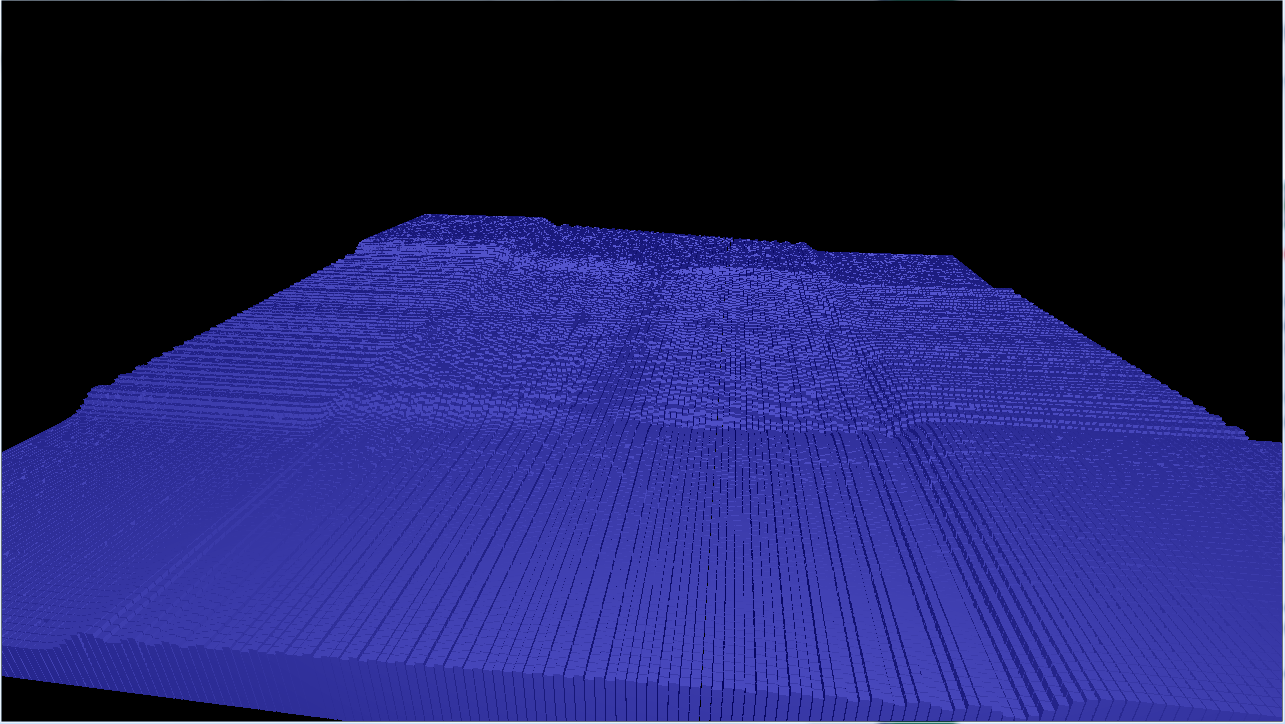
\includegraphics[width=0.5\textwidth]{../www/images/waterWaves}
\end{figure}

\begin{figure}[H]
    \caption{Wave Front}
    \label{fig:front}
    \centering
    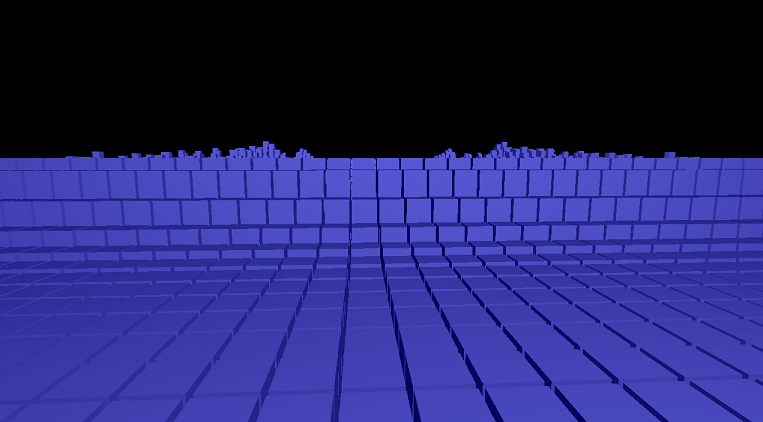
\includegraphics[width=0.5\textwidth]{../www/images/waveFront}
\end{figure}

Our implementation works well for modeling the surface movement of water as 
seen in figures \ref{fig:waves} and \ref{fig:front}. Ripples are clearly 
visible and can be seen propagating off of the boundaries as seen in figure 
\ref{fig:reflection}. Additionally, we were able to simulate object 
interaction; our cube is able to both effect and be affected by water.  The 
simulation also runs in real-time showing no significant slowdowns when run on 
our machine. While we were unable to implement a mesh over the surface of the 
water or any complex lighting techniques our focus was primarily on the 
simulation of water movement which our implementation successfully models.

\begin{figure}[H]
    \caption{Object Creating Water Displacement}
    \label{fig:displacement}
    \centering
    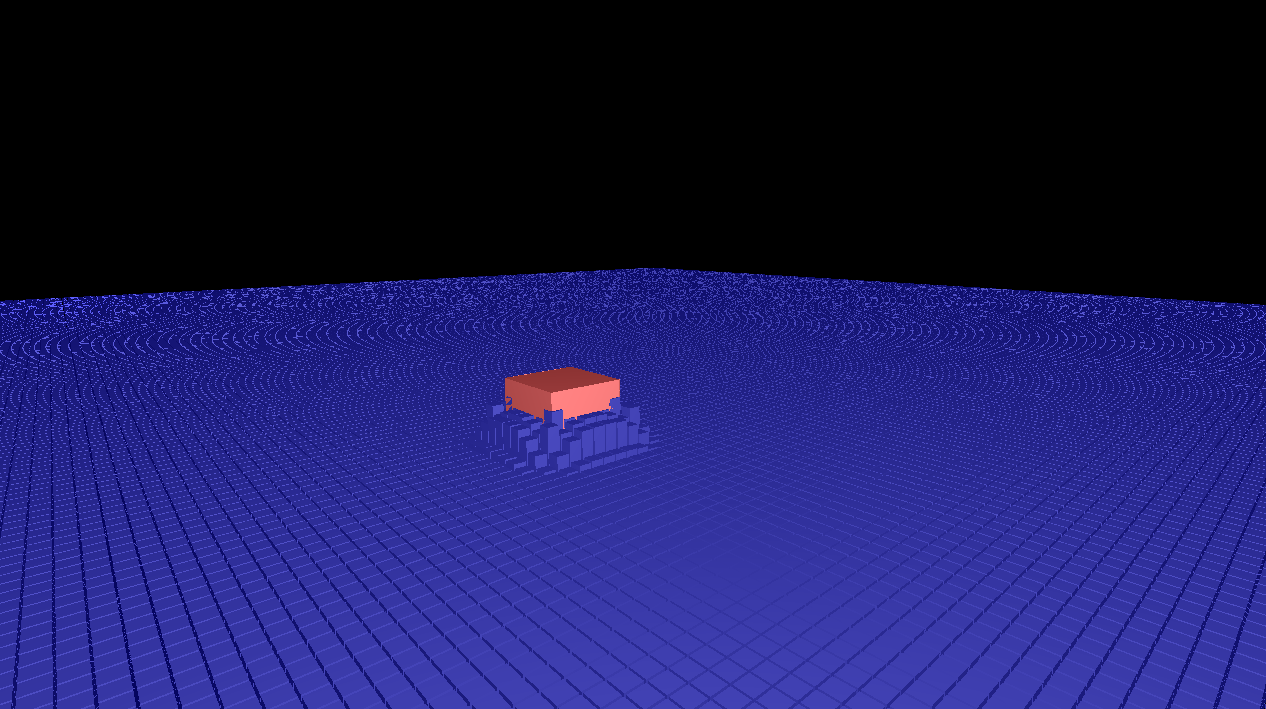
\includegraphics[width=0.5\textwidth]{../www/images/objectWaterDisplacement}
\end{figure}

Our implementation does have a few bugs, most notably both of our options for 
preventing feedback due to water displacement.  Setting the water level to the 
center of the cube creates large depressions or hills as the cube moved below 
or above the water’s surface as seen in figure \ref{fig:displacement}.  While 
the water was still able to cover and separate from the cube the simulation was 
more akin to oil then water due to the surface tension.  The other option 
produced realistic results when the water level was near level.  However if for 
some reason the cube was falling into water that was significantly higher or 
lower than average the interaction would occur far later or earlier than it 
should.  Other than this and minor problems due to our environmental constants, 
our simulation does perform as intended.

\section{Conclusion}

We investigated many ways of simulating water including wave particle systems, 
procedural fluids, and various height fields. Of all the available methods, we 
chose to implement a height field water simulation for two fundamental reasons, 
the ability to run it in real time and the ability to implement realistic 
object interactions. Our implementation works well for modeling the surface 
movement of water including ripples propagating off of the boundaries. It also 
works well for simulating object interactions that affect and are effected by 
the height field.

We were faced with challenges with feedback in the columns during multiple 
different interactions. The first interaction was in realistically creating 
reflections off of the boundaries of the height field and creating spontaneous 
ripples in the height field. Feedback was created due to two variables in these 
instances. One variable was the amount of damping that was being performed on 
the force applied to each column, the other was variance in the time step and 
how and when the force was applied. We originally calculated then immediately 
applied the force to a column and calculated it's new height in sequence 
causing some columns to behave strangely and also causing lots of feedback. 
This was solved by calculating the force on all columns then calculating the 
new height of all columns at a set interval. Although this was a simple 
mistake, it had very large impact on the performance of the height field. This 
solution coupled with small changes in the damping factor led a to a much more 
realistic simulation. Finding the correct damping factor was something we 
expected to be troublesome though because every source we found indicated the 
damping factor for height fields is not something that will be the same for 
every program.

In the future, this program could easily be expanded using techniques described 
in multiple articles. These expansions would similarly fall under two 
categories, wave motion and visual effects. Motion expansions such as adding 
breaking waves to a height field by creating a particle system for foam and 
water spray at the apex of a wave are quite possible. It would be a simple 
matter to identify a wave that is breaking using the curve between multiple 
columns at any given location on the height field and create and move the spray 
with that wave. Another straightforward motion addition would be implementing 
shallow water equations to simulate horizontal forces being applied to the 
system rather than vertical forces as we implemented.

Visually there is also a lot to expand upon. The first step would be 
transforming the columns of the height field to a curved surface. This would 
greatly simplify creating reflections, refractions, cloudiness, and caustics 
(the light disfigurations in a shallow body of water) using the normals found 
through the curving of the surface.

% References Section
% to add references, put them in the file references.bib in the same style
\nocite{*}
\printbibliography

\end{document}
